\section{ブリックをつかってみよう}
\subsection{使うブリックについて}
子どもIT未来塾で使うブリックについて紹介します。ブリックには番号が書いてあるので、表で確認しながら間違えて使わないように注意しましょう。\ref{sensor_intr}章のふろく:センサー紹介にはブリックについての詳しい説明が書いてあります。問題を解くときや自分で使ってみるときに参考にしましょう。\\

% 入出力
\newlength{\colA}
\setlength{\colA}{0.15\columnwidth}
% ブリック
\newlength{\colB}
\setlength{\colB}{0.15\columnwidth}
% 機能
\newlength{\colC}
\setlength{\colC}{0.3\columnwidth}
% 画像
\newlength{\colD}
\setlength{\colD}{0.2\columnwidth}
% 紹介ページ
\newlength{\colE}
\setlength{\colE}{0.07\columnwidth}

\begin{table}[H]
  \begin{tabular}{|p{\colA}|p{\colB}|p{\colC}|p{\colD}|p{\colE}|}
    \hline
	入出力 &ブリック / \par ブリック番号 & 機能 & 画像 & 紹介 \par ページ\\ \hline
	デジタル出力そうち & LED / \#101 & 
	\begin{minipage}[t]{\linewidth}
	%\smallskip
	\begin{itemize}
	 \item 順方向に電圧を加えると発光する
	 \item プログラムでは値が1のとき光り、値が0のとき消える
	\end{itemize}
	\smallskip
	\end{minipage} & 
    \begin{minipage}[t]{\linewidth}
    \smallskip
      \centering
      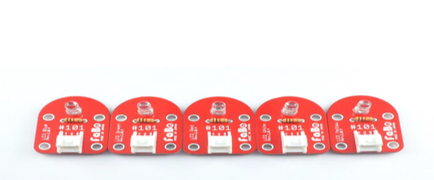
\includegraphics[width=\linewidth]{images/chap05/text05-img016.png}
      \smallskip
    \end{minipage} &
	\pageref{LED}\\ \cline{2-5}
	& 振動子 / \#105 & 
	\begin{minipage}[t]{\linewidth}
	%\smallskip
	\begin{itemize}
	 \item 電圧が加わると振動する
	 \item プログラムでは値が1のとき振動し、値が0のとき止まる
	\end{itemize}
	\smallskip
	\end{minipage} & 
    \begin{minipage}[t]{\linewidth}
    \smallskip
      \centering
      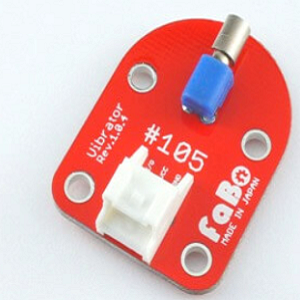
\includegraphics[width=0.8\linewidth]{images/chap05/text05-img017.png}
      \smallskip
    \end{minipage} &
    \pageref{vibrator}\\ \hline
    
    デジタル入力そうち & ボタン / \#103 & 
	\begin{minipage}[t]{\linewidth}
	%\smallskip
	\begin{itemize}
	 \item 押したり離したりしてONとOFFを切り替える。写真は黄色だが青や黒などの色もある。
	 \item プログラムではボタンが押されている間1、ボタンが押されていないと0が入力される
	\end{itemize}
	\smallskip
	\end{minipage} & 
    \begin{minipage}[t]{\linewidth}
    \smallskip
      \centering
      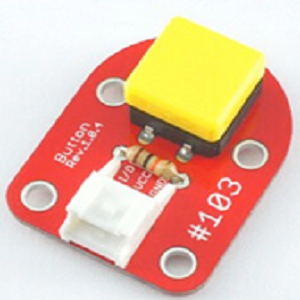
\includegraphics[width=0.8\linewidth]{images/chap05/text05-img028.png}
      \smallskip
    \end{minipage} &
	\pageref{button}\\ \cline{2-5}
	& 傾斜センサー / \#110 & 
	\begin{minipage}[t]{\linewidth}
	%\smallskip
	\begin{itemize}
	 \item かたむいているかを調べることができる
	 \item 傾くと1,傾いていないと0の値が入力される
	\end{itemize}
	\smallskip
	\end{minipage} & 
    \begin{minipage}[t]{\linewidth}
    \smallskip
    \smallskip
      \centering
      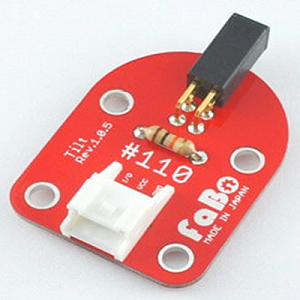
\includegraphics[width=0.8\linewidth]{images/chap05/text05-img018.png}
      \smallskip
    \end{minipage} &
    \pageref{tilt}\\ \hline   
  \end{tabular}
\end{table}

\begin{table}[H]
  \begin{tabular}{|p{\colA}|p{\colB}|p{\colC}|p{\colD}|p{\colE}|}
    \hline
	入出力 &ブリック/ \par ブリック番号 & 機能 & 画像 & 紹介ページ\\ \hline
    デジタル入力そうち & スイッチ / \#117 & 
	\begin{minipage}[t]{\linewidth}
	%\smallskip
	\begin{itemize}
	 \item ボタンと似ているが、ONのまま、OFFのままにできる
	 \item ●にスライドさせるとON、○にスライドさせるとOFFになる
	 \item ONのときは1,OFFのときは0が入力される
	\end{itemize}
	\smallskip
	\end{minipage} & 
    \begin{minipage}[t]{\linewidth}
    \smallskip
      \centering
      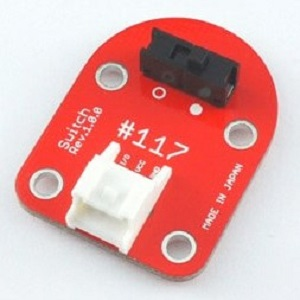
\includegraphics[width=0.8\linewidth]{images/chap05/text05-img019.jpg}
      \smallskip
    \end{minipage} &
    \pageref{switch}\\ \cline{2-5}
    & リミットスイッチ / \#107 & 
	\begin{minipage}[t]{\linewidth}
	%\smallskip
	\begin{itemize}
	 \item ボタンに似ている。銀の部分が押されているとON、押されていないとOFFになる
	 \item スイッチはONのときは1,OFFのときは0が入力される
	\end{itemize}
	\smallskip
	\end{minipage} & 
    \begin{minipage}[t]{\linewidth}
    \smallskip
      \centering
      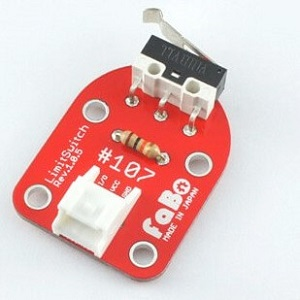
\includegraphics[width=0.8\linewidth]{images/chap05/text05-img020.jpg}
      \smallskip
    \end{minipage} &
    \pageref{lmswitch}\\ \hline   
    アナログ入力そうち & 感圧センサー / \#106 & 
	\begin{minipage}[t]{\linewidth}
	%\smallskip
	\begin{itemize}
	 \item 加えた力の大きさを調べることができる
	 \item 0〜1023の値が入力される。圧力が小さい時は値が大きく、圧力が大きい時は値が小さくなる。
	\end{itemize}
	\smallskip
	\end{minipage} & 
    \begin{minipage}[t]{\linewidth}
    \smallskip
      \centering
      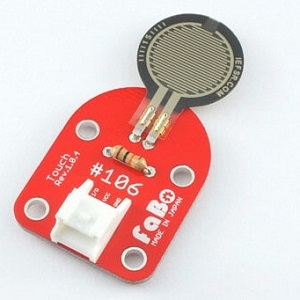
\includegraphics[width=0.8\linewidth]{images/chap05/text05-img021.jpg}
      \smallskip
    \end{minipage} &
    \pageref{touch}\\ \cline{2-5}
    & ボリューム / \#104 & 
	\begin{minipage}[t]{\linewidth}
	%\smallskip
	\begin{itemize}
	 \item じくをひねると電圧の大きさを変えることができる
	 \item 0〜1023の値が入力される。右に回すほど値が大きくなる。
	\end{itemize}
	\smallskip
	\end{minipage} & 
    \begin{minipage}[t]{\linewidth}
    \smallskip
      \centering
      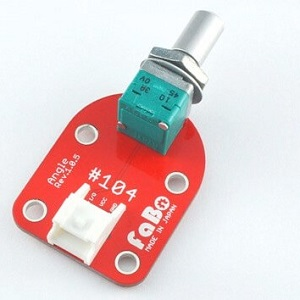
\includegraphics[width=0.8\linewidth]{images/chap05/text05-img022.jpg}
      \smallskip
    \end{minipage} &
    \pageref{volume}\\ \cline{2-5}
    & 距離センサー / \#116(番号は書いてありません) & 
	\begin{minipage}[t]{\linewidth}
	%\smallskip
	\begin{itemize}
	 \item 距離を測ることができる
	 \item 0〜1023の値が入力される。距離に変換する必要がある。
	\end{itemize}
	\smallskip
	\end{minipage} & 
    \begin{minipage}[t]{\linewidth}
    \smallskip
      \centering
      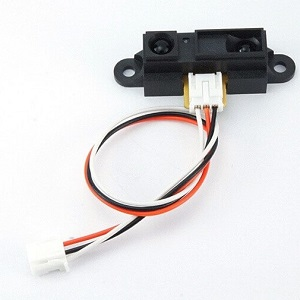
\includegraphics[width=0.8\linewidth]{images/chap05/text05-img023.jpg}
      \smallskip
    \end{minipage} &
    \pageref{distance}\\ \hline   
  \end{tabular}
\end{table}

\begin{table}[H]
  \begin{tabular}{|p{\colA}|p{\colB}|p{\colC}|p{\colD}|p{\colE}|}
    \hline
	入出力 &ブリック/ \par ブリック番号 & 機能 & 画像 & 紹介ページ\\ \hline
    デジタル入力そうち & 照度センサー / \#109 & 
	\begin{minipage}[t]{\linewidth}
	%\smallskip
	\begin{itemize}
	 \item 明るさの変化を測ることができる
	 \item 0〜1023の値が入力される。暗いほど値が大きくなる。
	\end{itemize}
	\smallskip
	\end{minipage} & 
    \begin{minipage}[t]{\linewidth}
    \smallskip
      \centering
      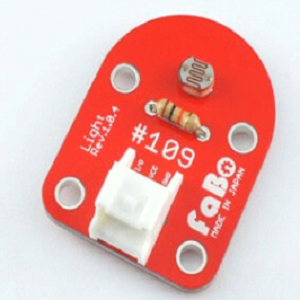
\includegraphics[width=0.8\linewidth]{images/chap05/text05-img024.png}
      \smallskip
    \end{minipage} &
    \pageref{light}\\ \hline
    その他 & ゆうきELディスプレイ / \#214 & 
	\begin{minipage}[t]{\linewidth}
	%\smallskip
	\begin{itemize}
	 \item 文字を画面に表示させることができる(アルファベットと記号のみ)
	 \item oled “文字”で表示する
	\end{itemize}
	\smallskip
	\end{minipage} & 
    \begin{minipage}[t]{\linewidth}
    \smallskip
      \centering
      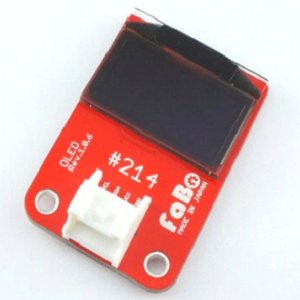
\includegraphics[width=0.8\linewidth]{images/chap05/text05-img025.png}
      \smallskip
    \end{minipage} &
    \pageref{oled}\\ \hline
    \end{tabular}
\end{table}